\documentclass[addpoints,11pt,a4paper]{exam}
\usepackage{anysize}
\marginsize{1cm}{2cm}{.5cm}{1cm}
\usepackage[utf8]{inputenc}
\usepackage[magyar]{babel}
\usepackage{t1enc}
\usepackage{nicefrac}
\usepackage{siunitx}
\usepackage{multicol}
\usepackage{mailmerge}
\usepackage{amsmath}
\usepackage{amssymb,wasysym}
\usepackage{dsfont}
\pagestyle{empty}
\pointname{ pont}
\usepackage{multicol}

\usepackage{tikz}
\usetikzlibrary{patterns}
\begin{document}
	
	
	\begin{questions}
		\question A fémezüstből megvilágítás hatására kilépő elektron kilépési munkája $0,69 \mathrm{~aJ}$.  
		\begin{parts}
			\part Legalább mekkora legyen annak a fénynek a frekvenciája, amelynek hatására az elektron kiléphet az ezüst felületéről?
			\part Milyen fényről lehet szó: infravörös, látható vagy ultraibolya fényről?
		\end{parts}
		
		\question Vizsgáljunk egy $0,02\mathrm{~W}$ teljesítményű, $630\cdot 10^{-9}\mathrm{~m}$ hullámhosszon sugárzó héliumneon lézert!
		\begin{parts}
			\part Határozza meg a lézer által kibocsátott fény egy fotonjának energiáját!
			\part Határozza meg a fényforrás által két másodperc alatt kibocsátott fotonok számát! 
		\end{parts}
		
		\question A hidrogénatom energiaszintjeit az  $E_n=-\dfrac{2,2}{n^{2}}\mathrm{~aJ}$ összefüggéssel írhatjuk le. (Ahol n= 1,2,3,… pozitív egész szám, amely a különböző energiaszinteket jelöli.) Mekkora annak az elektromágneses hullámnak a hullámhossza, amelyet a hidrogén akkor sugároz ki, amikor egy elektronja a 2. energiaszintről a legmélyebb energiaszintre ugrik?
		
		\question Tegyük fel, hogy egy hidrogénatom fotont bocsát ki, miközben elektronja az $n = 5$ főkvantumszámmal jelzett állapotból az $n = 3$ főkvantumszámmal jelzett állapotba jut. Az így kibocsátott fotont elnyeli egy másik hidrogénatom, amely így ionizálódik. Hányas főkvantumszámú állapotban lehetett az ionizált hidrogénatom elektronja a foton elnyelése előtt? A hidrogénatom elektronjának energiája az $n$ főkvantumszámmal jelzett állapotban $E_n = -\dfrac{13,6}{n^{2}}\mathrm{~eV}$. 
		
		\question Egy $10\mathrm{~W} $ teljesítményű fényforrás $450\mathrm{~nm}$ hullámhosszúságú kék fényt bocsát ki.
		\begin{parts}
			\part Mekkora egy foton energiája?
			\part Hány foton hagyja el a fényforrást 1 perc alatt? 
		\end{parts}
		 
		 \question A fényelektromos jelenség során fotonok elektronokat löknek ki egy ezüstlemezből. Az alábbi táblázat a becsapódó fotonok energiáját és a kilépő elektronok mozgási energiáját tartalmazza. (Ez utóbbit feszültségmérés segítségével határozták meg.) A táblázatból egy adat hiányzik.
		 \begin{center}
		 	$\begin{array}{|c|c|c|c|c|c|c|}
		 	\hline \text { foton energiája - }(\mathrm{eV}) & 5,12 & 5,88 & & 6,92 & 7,55 & 7,92 \\
		 	\hline \text { elektron energiája - }(\mathrm{eV}) & 0,41 & 1,12 & 1,52 & 2,17 & 2,77 & 3,20 \\
		 	\hline
		 \end{array}$
		 \end{center}
		 \begin{parts}
		 	\part Ábrázolja grafikusan a kilépő elektronok energiáját a fotonok energiájának függvényében!  
		 	\part A fenti adatok segítségével határozza meg, hogy mennyi a kilépési munka az ezüst esetében!  
		 	\part Legfeljebb mekkora lehet a fotonok hullámhossza, hogy az elektronkilökés lejátszódjon?  
		 	\part Számítással vagy a grafikon alapján adja meg a táblázatból hiányzó adatot! 
		 \end{parts}
		 \begin{center}
		 	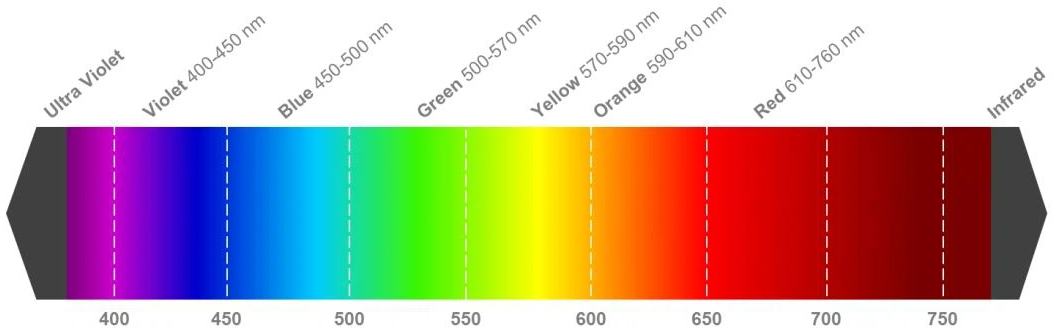
\includegraphics[width=\textwidth]{abra01}
		 \end{center}
	\begin{center}
			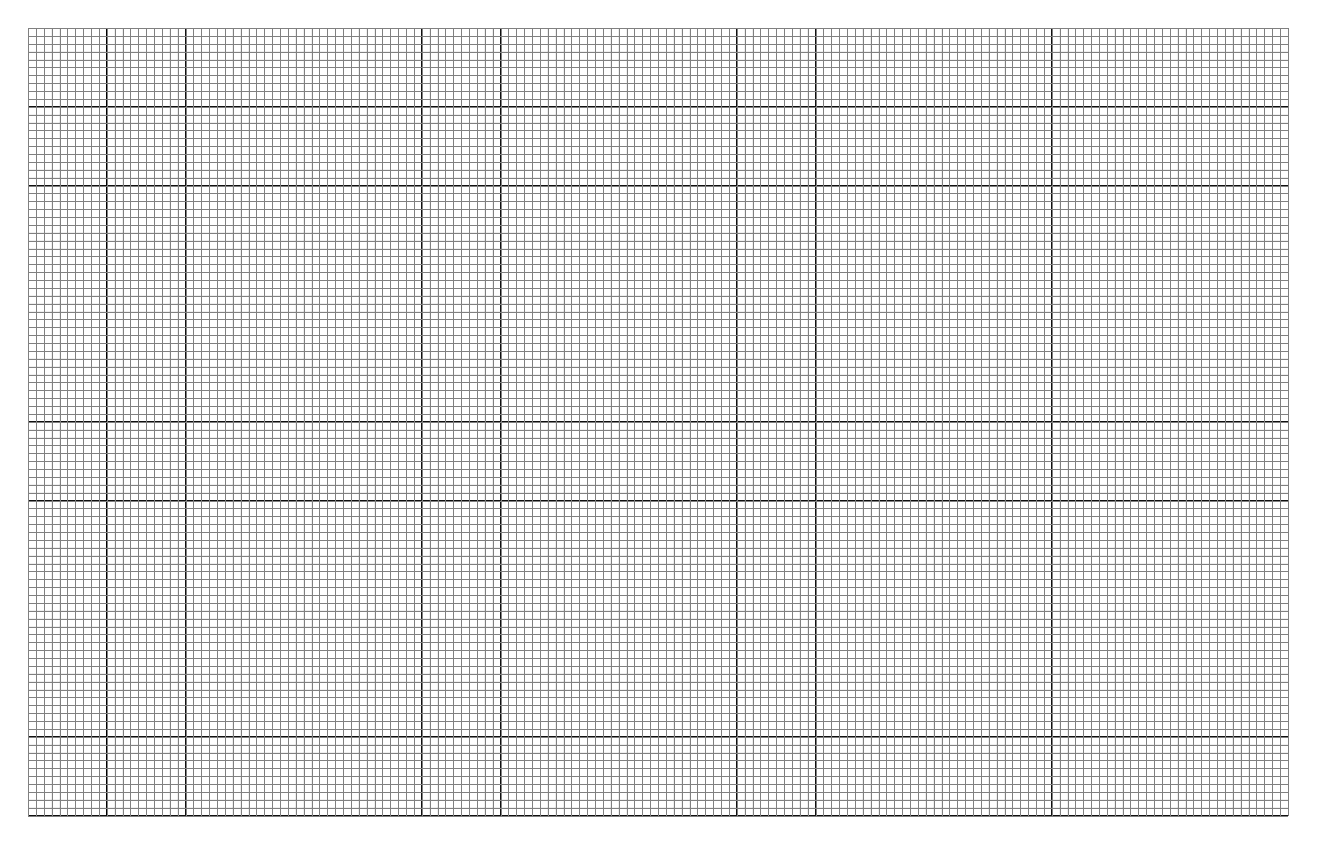
\begin{tikzpicture}[x=1mm, y=1mm, dotted/.style={pattern=dots}]
			
			\draw[step=10mm, line width=0.15mm, dotted] (0,0) grid (160mm,100mm);
			\draw[step=1mm, line width=0.035mm, dotted, gray] (0,0) grid (160mm,100mm);
		\end{tikzpicture}
	\end{center}
		  
	\end{questions}
\end{document}